\section{Introduction}

\subsection{Motivation}

% Frame with plain text
\begin{frame}{Motivation}
  \begin{itemize}
    \item Rise of World Wide Web led to better collaboration between researchers
    \item Place to meet and exchange information
          %researchers in particular from all over the world can collaborate more easily 
    \item This led to the rise of online Communities of Practice (CoP)
          %what Cops are will be discussed in more detail later.
    \item Success of CoP relies on success factors, which are changing over time
    \item It is difficult to measure and evaluate them
          \begin{itemize}
            \item Domain specific success factors
            \item Time consuming
            \item Require data-management experts %which especially small CoPs lack
          \end{itemize}
  \end{itemize}
\end{frame}


\begin{frame}{Motivation}
  %this is why some continuous success modeling systems have been developed
  %however, the problem is that
  \begin{columns}
    \begin{column}[]{0.5\textwidth}

      Current success modeling systems
      \begin{itemize}
        \item Complicated %and require technical know-how
        \item Not optimized for collaboration
        \item Do not take mobility into consideration
      \end{itemize}

    \end{column}
    \begin{column}[]{0.5\textwidth}
      Chat platforms are used for information exchange
      \begin{itemize}
        \item Intuitive
        \item Collaboration
        \item Optimized for mobile devices
      \end{itemize}
      %This shows how chat platforms could adress the aforementionted issues
    \end{column}
  \end{columns}

\end{frame}


\subsection{Thesis Goals}

\begin{frame}{Thesis Goals}
  \begin{itemize}
    \item Design a chatbot for success modeling and visualizations
    \item Interface which communicates between
          \begin{itemize}
            \item End-User
            \item Existing CIS
                  %Especially for visualizations of success factors of the Community
          \end{itemize}
    \item Bot should communicate wit MobSOS (CCA) %framework
    \item Should be deployed with the Social Bot Framework
  \end{itemize}
\end{frame}

%------------------------------------------------

% Start a new section (text is displayed on top of a frame)
\section{State of the Art}

\subsection{Social Bots}
\begin{frame}{Social Bots and Chatbots}
  \begin{block}{Definition}
    ``A social bot is a computer algorithm that automatically produces content and interacts with humans on social media, \dots'' \cite{FVD*16b}
  \end{block}
\end{frame}
\begin{frame}{Social Bots and Chatbots}
  \begin{block}{Definition}
    ``A social bot is a computer algorithm that automatically produces content and interacts with humans on social media, \dots'' \cite{FVD*16b}
  \end{block}
  \begin{itemize}
    \item Can be used for automation of daily tasks %e.g. Alexa Smart Home, Shopping lists Reminders
    \item Users interact with Bots through voice or chat %in the case of chat: Chatbots
    \item Better user experience as more intuitive to use
  \end{itemize}
\end{frame}

\subsection{Succes in Communities of Practice}
\begin{frame}{Communities of Practice}
  \begin{block}{Definition}
    ``Communities of practice are groups of people who share a concern or a
    passion for something they do and learn how to do it better as they interact regularly.'' \cite{Weng98}
  \end{block}
\end{frame}

\begin{frame}{Communities of Practice}
  \begin{block}{Definition}
    ``Communities of practice are groups of people who share a concern or a
    passion for something they do and learn how to do it better as they interact regularly.'' \cite{Weng98}
  \end{block}
  \begin{itemize}
    \item Community consisting of members studying a particular domain
    \item Members of a Community of Practice:
          \begin{itemize}
            \item Researchers
            \item Professionals
            \item Students
            \item Hobbyists
          \end{itemize} %DBIS and ACIS as an example????
  \end{itemize}
\end{frame}


\begin{frame}{Communities of Practice}
  \begin{itemize}
    \item Members of different degrees of
          \begin{itemize}
            \item Knowledge %Researchers > students
            \item Interest %Professionals > Hobbyists
            \item Contribution
          \end{itemize}
    \item Based on Contribution we discern between
          \begin{itemize}
            \item Core Members %do most of the contribution 
            \item Lurkers %only consume but almost no contribution
                  %study on open Source found that for random projects 22percent contribute. For the top 500 projects: ~90percent don't contribute -> 1% (90-9-1) rule
          \end{itemize}
    \item Members do not have to belong to the same organization
    \item Share their work through social interaction e.g. online Social Networks %in this case we also talk about an online CoP
    \item Communities contain sub-commmunities which can be overlapping
  \end{itemize}
\end{frame}

\begin{frame}{Measurement of Success}
  \begin{itemize}
    \item Communities of Practice need to be aware of their success
          \begin{itemize}
            \item Improve their work
            \item Adjust to current trends
          \end{itemize}
          %Success seems to be a very abstract metric so in order to measure it we build a success model
    \item Measurement of Success through a \emph{Success Model}
    \item Success model distinct for each Community of Practice %as CoPs are very diversen and informal structures with permeable boundaries

  \end{itemize}
\end{frame}
\begin{frame}{Success Model}
  \begin{figure}[!h]
    \centering
    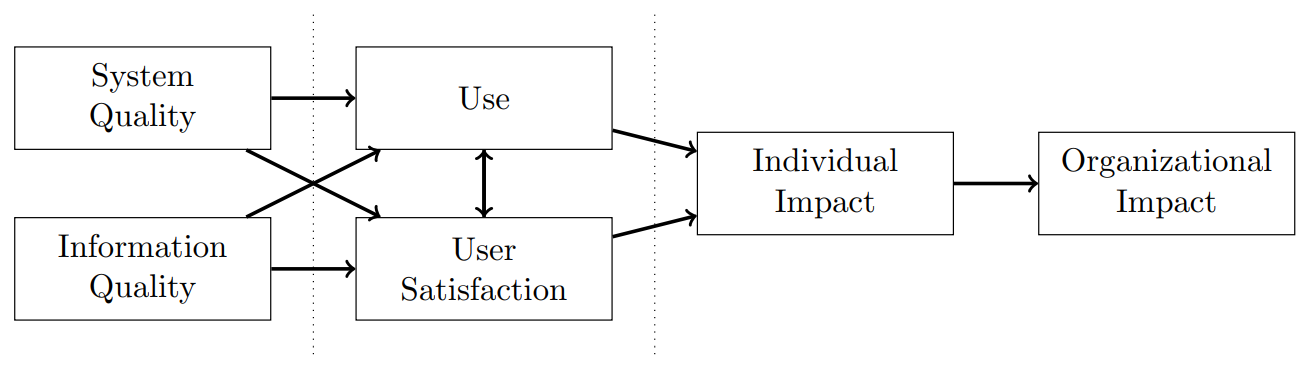
\includegraphics[width=0.7\textwidth]{related_work/deloneMclean.png}
    \caption{Community Information Systems Success Model by DeLone and McLean \cite{DeMc92}}
    %13!!!!
  \end{figure}
  MobSOS success model is based on this model
\end{frame}

\begin{frame}{MobSOS}

  \begin{itemize}
    \item Core Component of las2peer
    \item Monitors las2peer services
    \item MobSOS Continuous Community Analytics extends MobSOS
          \begin{itemize}
            \item Provides visualizations of MobSOS data
            \item Ability to dynamically add databases and Mediabases
          \end{itemize}
  \end{itemize}
  %The MobSOS cca also allows the addition of Mediabases, which can be used to gather data produced outside the las2peer environment
\end{frame}

\begin{frame}{Mediabase Schema}
  \begin{figure}[h]
    \centering
    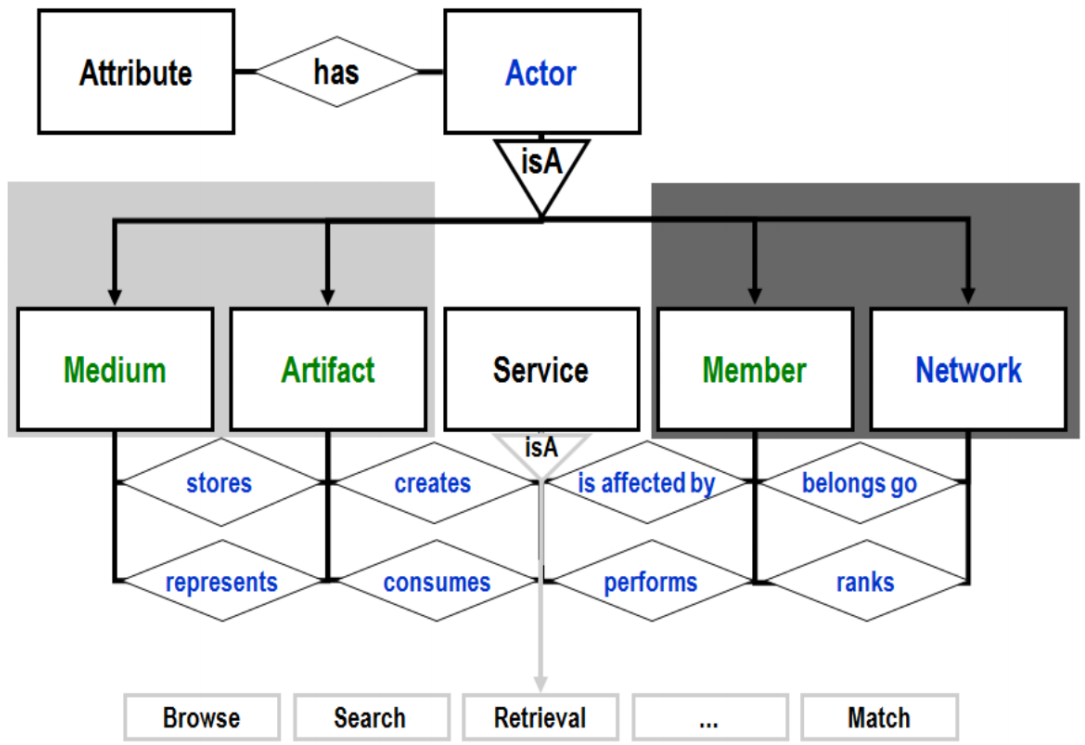
\includegraphics[height=0.89\textheight]{related_work/mediabase.png}
    \caption{Mediabase Overview \cite{Klam10e}}
  \end{figure}
\end{frame}

\begin{frame}{Mediabase Concept}
  Mediabase includes
  \begin{itemize}
    \item Backend database (DB2 or MySQL)
    \item Crawler scripts
    \item Monitoring processes
    \item Frontend for user interactions
  \end{itemize}
\end{frame}

\section{Concept}
\subsection{Use Case}
\begin{frame}{Mensa Communities}
  \begin{itemize}
    \item Community of people frequently visiting the mensa
    \item Community consists of students and university employees
    \item Similar to the concept of Community of Practice %share a concern: food at the canteen. And Interact regularly: Students argumenting on which mensa is the best?? Freqwuent visits to mensa
    \item Different community levels:
          \begin{itemize}
            \item Top level: all mensa frequenteers in Germany
            \item Intermediate level: all mensa frequenteers for a University
            \item Low level: individual circle of friends, which frequent the canteen together %Members can belong to different circles of friends->overlapping
          \end{itemize}
  \end{itemize}
\end{frame}



\begin{frame}{Mensa Bot}
  For this community a chatbot is designed, which can be used to
  \begin{itemize}
    \item Get the menu for a canteen
    \item Rate meals
    \item Query success visualizations for meals, canteens and other success metrics, which can be designed by the community
  \end{itemize}
  The chatbot is deployed with Slack.
\end{frame}

\begin{frame}{Use case diagram for the Chatbot}
  \begin{figure}
    \centering
    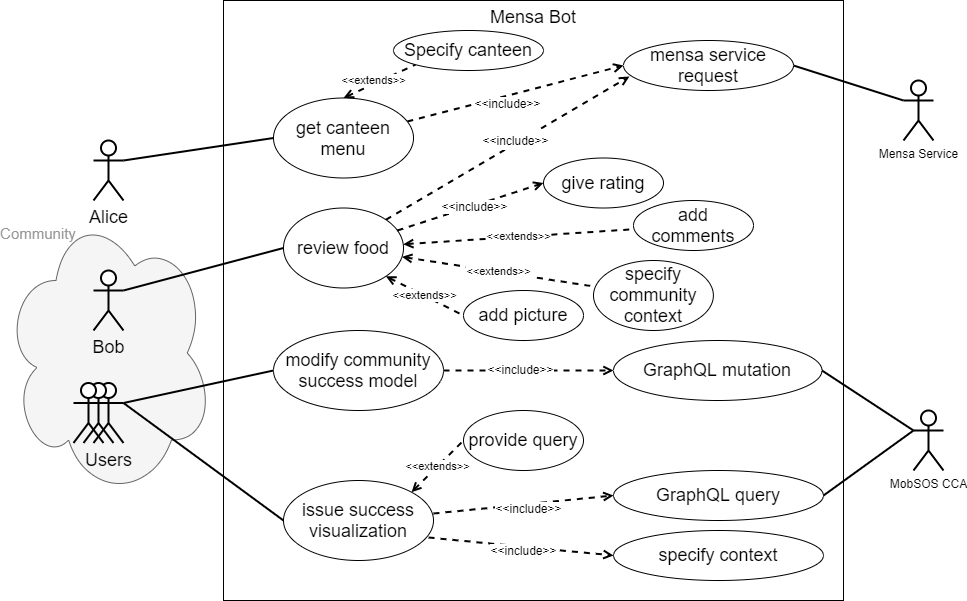
\includegraphics[height=0.85\textheight]{concept/usecase.png}

  \end{figure}
\end{frame}

\subsection{System overview}

\begin{frame}{System overview}
  \begin{figure}
    \centering
    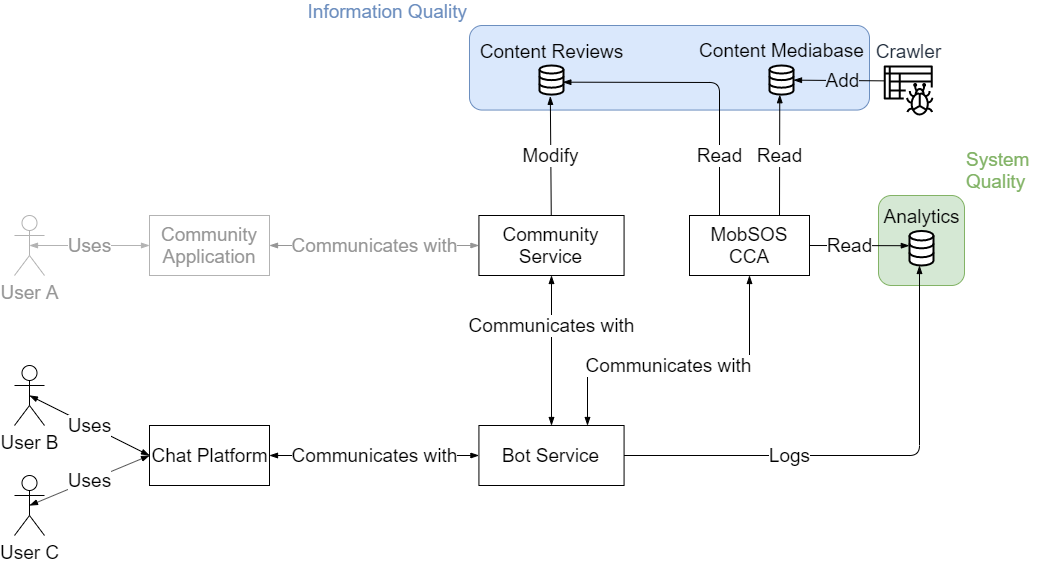
\includegraphics[height=0.85\textheight]{realization/Component_Diagramm.png}

    \label{fig:sytsemOverview}
  \end{figure}
\end{frame}

\section{Realization}

\begin{frame}
  \begin{figure}
    \centering
    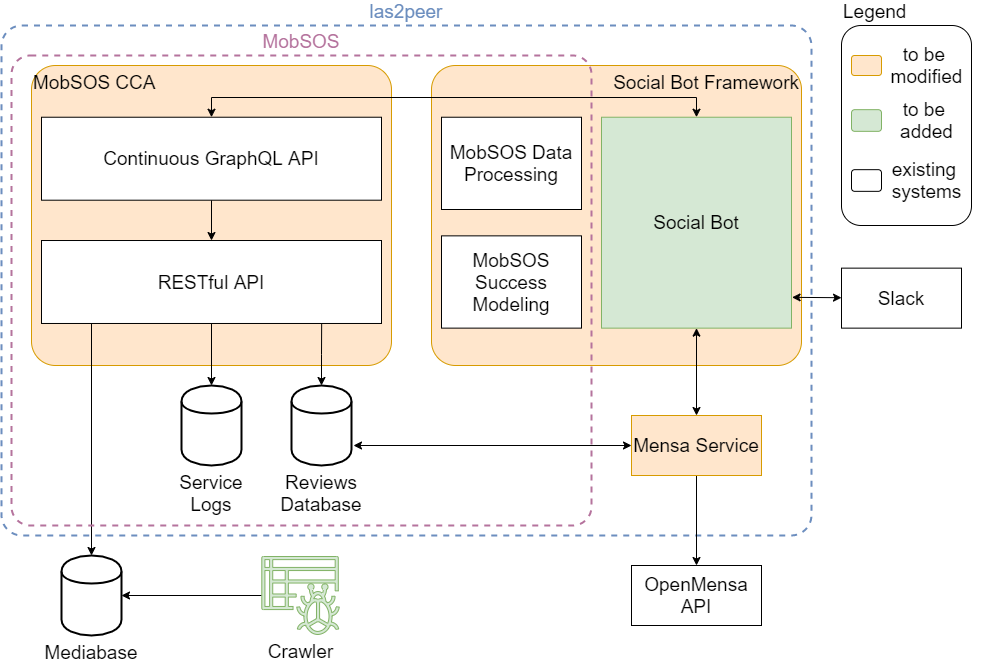
\includegraphics[height=0.9\textheight]{realization/components_overview.png}
    \caption{Overview of the different components}
    \label{fig:componentsOverview}
  \end{figure}
\end{frame}

\begin{frame}{Example use of community Service with the Bot}
  \begin{figure}
    \centering
    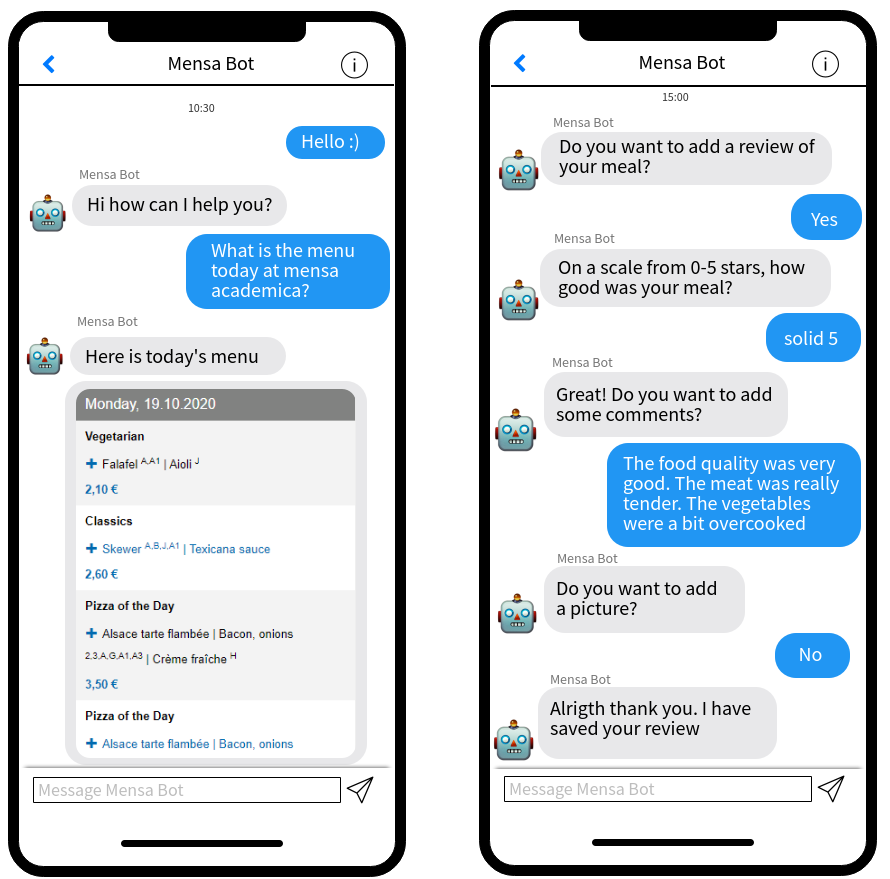
\includegraphics[height=0.9\textheight]{realization/chat_mockup.png}

  \end{figure}
\end{frame}

\begin{frame}{Example of a visualization request}
  \begin{figure}
    \centering
    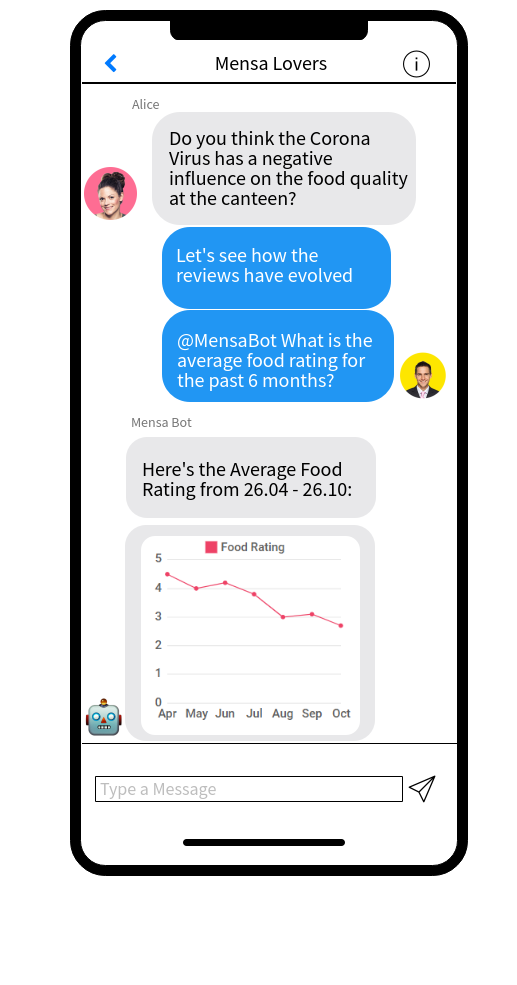
\includegraphics[height=\textheight]{realization/visual_req.png}

    \label{fig:visualReq}
  \end{figure}
\end{frame}

\section{Evaluation}

\begin{frame}{Thesis questions}
  \begin{itemize}
    \item Does the use of chatbots increase the success awareness of the community?
    \item Does it increase collaboration between members?
    \item Does it improve the user experience in terms of mobility?
  \end{itemize}
\end{frame}

\begin{frame}{Overview}
  \begin{itemize}
    \item Create a mensa community
    \item Members will be students and university employees
          \begin{itemize}
            \item need to frequent the mensa regularly %note here that this might be difficult right now cos covid
          \end{itemize}
    \item Slack Bot deployed to ACIS Slack for collecting reviews (falls möglich, was meinst du?)
  \end{itemize}
\end{frame}

\begin{frame}{Community Service Phase}
  \begin{itemize}
    \item Evaluate the usability of the bot for getting menu and making reviews
    \item Volonteers will be acting as community members
    \item Members will join a new Mensa Slack group
    \item The chatbot is included in a group channel
          \begin{itemize}
            \item can be used to query menu
          \end{itemize}
    \item Members are asked to make a food review by Direct Message with the bot
    \item Hand out questionnaire
  \end{itemize}
\end{frame}

\begin{frame}{Success Modeling Phase}
  \begin{itemize}
    \item Evaluate the collaboration aspect of the bot
    \item Preferably same volonteers as first phase %maybe some new features were added in the first phase which they can now try out...
    \item Divide into groups of 2-3 students
          \begin{itemize}
            \item make visualization requests
            \item update the success model
          \end{itemize}
    \item Fill out questionnaire
  \end{itemize}
\end{frame}

\section{Project Plan}

\begin{frame}
  \begin{figure}
    \centering
    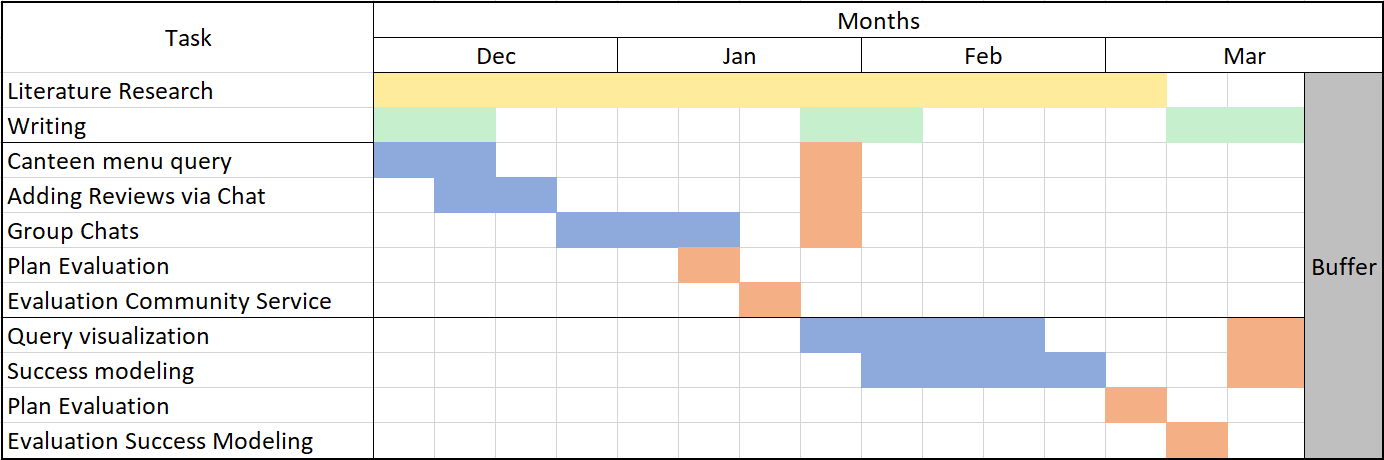
\includegraphics[width=0.89\textwidth]{project_plan/projectplan.png}

    \label{fig:visualReq}
  \end{figure}
\end{frame}